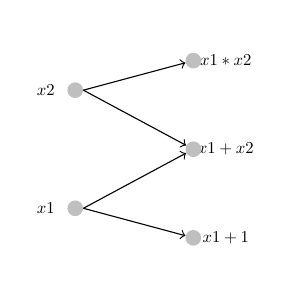
\begin{tikzpicture}[scale = 0.75,
         arrow/.style={->,black},
         set name/.style={font=\color{myblue}\tiny\bfseries\sf},
         set/.style={thick, myblue},
         every node/.style={scale=0.6,circle},
         font=\sf
      ]
   \node (x1L) at (0.5, 0.0) {$x1$};
   \node (x2L) at (0.5, 2.0) {$x2$};
   \node (y1L) at (3.55, -0.5) {$x1 + 1$};
   \node (y2L) at (3.55, 1.0) {$x1 + x2$};
   \node (y3L) at (3.55, 2.5) {$x1 * x2$};

   \node[fill=lightgray] (x1) at (1.0, 0.0) {};
   \node[fill=lightgray] (x2) at (1.0, 2.0) {};
   \node[fill=lightgray] (y1) at (3.0 , -0.5) {};
   \node[fill=lightgray] (y2) at (3.0 , 1.0) {};
   \node[fill=lightgray] (y3) at (3.0 , 2.5) {};

   \begin{scope}[arrow]
      \draw (x1.east) -- (y1);
      \draw (x1.east) -- (y2);
      \draw (x2.east) -- (y2);
      \draw (x2.east) -- (y3);
   \end{scope}
\end{tikzpicture}